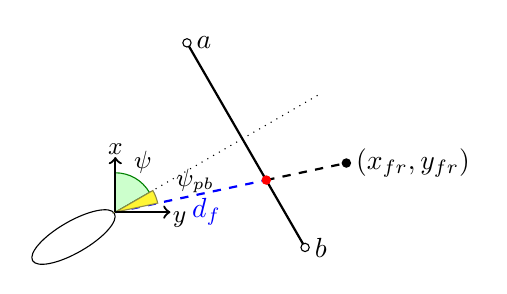
\begin{tikzpicture}

%AUV
\draw[rotate=30] (1.8,-1) ellipse (0.6 and 0.2);

%Pier
\path (3.5,2.5) coordinate (a);
\path (a)++(-60:3) coordinate (b);
\draw[thick] (a) -- (b);
\filldraw[fill=white, draw=black](a) circle(1.5pt) node[right]{$a$};
\filldraw[fill=white, draw=black](b) circle(1.5pt) node[right]{$b$};

%Aux
\path (2.59,0.35) coordinate (f);
\draw[dotted] (f) -- ++(30:3);
\draw[dashed, thick, blue] (f) -- ++(12:1.96) node[midway, below, xshift=2mm, yshift=1mm] {$d_f$};
\draw[dashed, thick] (f)++(12:1.96) -- ++(12:1.04);
%Angles
\filldraw[fill=green!20,draw=green!50!black] (f) -- ++(0,0.5) arc (90:30:0.5) node[midway, xshift=1mm, yshift=2mm] {\small $\psi$} -- cycle; 
\filldraw[fill=yellow!80,draw=yellow!50!black] (f) -- ++(30:0.55) arc (30:12:0.55) node[midway, xshift=5mm, yshift=2mm] {\small $\psi_{pb}$} -- cycle;

%Points
\filldraw[black](f)++(12:3) circle(1.5pt) node[right]{$\left(x_{fr},y_{fr}\right)$};
\filldraw[red](f)++(12:1.96) circle(1.5pt);

%Axis
\draw[thick,->] (f) -- ++(0.7,0) node[right, xshift=-1mm, yshift=-1mm] {\small $y$};
\draw[thick,->] (f) -- ++(0,0.7) node[above, yshift=-1mm] {\small $x$};

\end{tikzpicture}